\documentclass[12pt,a4paper]{article}

\usepackage{fontspec}
\setmainfont{Arial}
\usepackage[brazil]{babel}
\usepackage{geometry}
\geometry{top=2.5cm,bottom=2.5cm,left=3cm,right=3cm}
\usepackage{setspace}
\setstretch{1.35}
\usepackage{graphicx}
\graphicspath{{figuras/}}
\usepackage{booktabs}
\usepackage{tabularx}
\usepackage{longtable}
\usepackage{array}
\usepackage{float}
\usepackage{caption}
\usepackage{subcaption}
\usepackage{pdflscape}
\usepackage{tikz}
\usetikzlibrary{arrows.meta,positioning,fit,shapes.geometric}
\usepackage{amsmath}
\usepackage{enumitem}
\usepackage{xcolor}
\usepackage{titlesec}
\usepackage{fancyhdr}
\usepackage{lastpage}
\usepackage{ragged2e}
\usepackage{microtype}
\usepackage{xurl}
\usepackage{hyperref}

\definecolor{aripsbrown}{HTML}{76573F}
\definecolor{aripsgreen}{HTML}{59651F}
\definecolor{aripsgold}{HTML}{DDAF4D}
\definecolor{aripscream}{HTML}{F4F1E9}
\definecolor{aripsink}{HTML}{22241D}

\hypersetup{
  colorlinks=true,
  linkcolor=aripsbrown,
  citecolor=aripsgreen,
  urlcolor=aripsbrown,
  pdftitle={Relatório Final PIBIC -- ARIPS},
  pdfsubject={Desenvolvimento de um chatbot inteligente para auxílio na regulagem de implementos de preparo de solo}
}

\titleformat{\section}{\bfseries\large}{\thesection}{0.75em}{}
\titleformat{\subsection}{\bfseries\normalsize}{\thesubsection}{0.75em}{}
\titlespacing*{\section}{0pt}{1.2em}{0.6em}
\titlespacing*{\subsection}{0pt}{1em}{0.4em}
\setlist{nosep,leftmargin=1.1cm}
\setlength{\parindent}{1.25cm}
\setlength{\parskip}{0.15em}
\captionsetup{font=small,labelfont=bf,justification=centering}

\pagestyle{fancy}
\fancyhf{}
\fancyfoot[C]{\thepage}
\renewcommand{\headrulewidth}{0pt}

\newcommand{\fonteautor}{\par\vspace{-0.35em}{\centering\footnotesize Fonte: elaborado pelo autor (2026).\par}}
\newcommand{\sigla}[1]{\textsc{#1}}

\begin{document}
\justifying
\hypersetup{pageanchor=false}

% Capa construída a partir do modelo institucional. Os nomes são omitidos conforme a orientação do modelo.
\begin{titlepage}
  \thispagestyle{empty}
  \begin{center}
    
\includegraphics[height=3.0cm]{ufs.jpeg}\par
    \vspace{0.4cm}
    {\bfseries UNIVERSIDADE FEDERAL DE SERGIPE\par}
    {PRÓ-REITORIA DE PÓS-GRADUAÇÃO E PESQUISA\par}
    {COORDENAÇÃO DE PESQUISA\par}
    \vspace{0.55cm}
    {\bfseries PROGRAMA INSTITUCIONAL DE BOLSAS DE INICIAÇÃO CIENTÍFICA\par}
    {PIBIC 2025/2026\par}
    \vfill
    {\bfseries\Large DESENVOLVIMENTO DE UM CHATBOT INTELIGENTE PARA AUXÍLIO NA REGULAGEM DE IMPLEMENTOS DE PREPARO DE SOLO\par}
    \vspace{0.7cm}
    {\large Plano de trabalho: Abordagem Técnico-Científica com Validação Progressiva\par}
    \vfill
    {\bfseries\Large RELATÓRIO FINAL\par}
    \vspace{1.1cm}
    {Vigência do plano: setembro de 2025 a agosto de 2026\par}
    \vspace{1.5cm}
    {São Cristóvão -- SE\par}
    {2026\par}
  \end{center}
\end{titlepage}

\hypersetup{pageanchor=true}
\pagenumbering{roman}
\setcounter{page}{1}
\tableofcontents
\clearpage
\pagenumbering{arabic}

\section{Introdução}

O preparo do solo constitui uma das etapas que mais interferem nas condições físicas para a implantação de uma cultura. A seleção do implemento, a potência disponível, a profundidade, a umidade e o tempo para concluir a operação formam um conjunto de variáveis que não deve ser analisado de maneira isolada. A movimentação excessiva pode pulverizar a camada superficial, aumentar a suscetibilidade à erosão e favorecer a compactação em camadas mais profundas, enquanto a seleção inadequada do conjunto trator--implemento pode reduzir a capacidade operacional e elevar o consumo de energia \cite{embrapa_melancia,embrapa_feijao}. Dessa forma, a regulagem não é apenas uma escolha mecânica, mas uma decisão que relaciona solo, máquina, operação e planejamento.

Esse problema também se encontra em um ambiente marcado pela desigualdade no acesso à orientação técnica. No Censo Agropecuário de 2017, somente 20,1\% dos produtores declararam receber assistência técnica, proporção inferior aos 22\% observados em 2006 \cite{ibge2019,ibge2017}. Ao mesmo tempo, o número de tratores nos estabelecimentos cresceu 49,9\% no mesmo intervalo e alcançou 1,22 milhão de unidades \cite{ibge2019}. Esses dados mostram que a presença da máquina não garante, por si só, o acesso ao conhecimento necessário para sua utilização. Parte da informação permanece dispersa em anuários, catálogos de fabricantes e manuais extensos, muitas vezes organizados em tabelas que não permitem uma consulta rápida durante o planejamento da operação.

Dentro desse contexto, foi desenvolvido o ARIPS, sigla adotada para a aplicação cujo propósito é auxiliar, de forma inteligente, a regulagem de implementos de preparo do solo. A solução reúne uma base técnica de tratores, arados e grades, um mecanismo de recomendação, um módulo de planejamento operacional e um assistente conversacional. A proposta não foi substituir o engenheiro agrícola, o agrônomo ou o manual do fabricante, mas organizar o conhecimento disponível e fornecer uma primeira orientação rastreável, que possa ser confirmada pelo responsável técnico e por uma passagem de teste no campo.

O desenvolvimento exigiu relacionar conteúdos de mecanização agrícola, processamento de documentos, bancos de dados, engenharia de software e aprendizagem de máquina. Essa relação encontra fundamento no pensamento complexo de Edgar Morin, para quem o conhecimento pertinente precisa reconhecer as ligações entre as partes e o contexto no qual elas se encontram \cite{morin2000,morin2015}. No caso estudado, potência, largura, profundidade, tipo de solo e umidade não são informações independentes. Uma recomendação coerente surge da articulação entre esses dados e do reconhecimento das incertezas existentes nos catálogos e nas condições reais de campo.

Ao mesmo tempo, o pensamento computacional orientou a transformação do problema amplo em partes menores. Wing descreve essa forma de raciocínio como o uso de conceitos da computação para resolver problemas, projetar sistemas e compreender comportamentos, destacando a decomposição e a abstração como práticas centrais \cite{wing2006}. No projeto, o processo foi dividido em aquisição dos documentos, extração, limpeza, normalização, persistência, treinamento, recomendação, interação e validação. Depois, essas partes foram integradas em uma aplicação única. Essa divisão permitiu testar cada etapa e localizar erros sem perder a visão do resultado final.

Assim, este relatório apresenta a metodologia empregada na construção da base técnica, no desenvolvimento da aplicação e no treinamento do modelo. Também descreve a arquitetura adotada, os desafios do chatbot, os resultados computacionais alcançados e as limitações que ainda precisam ser enfrentadas em uma validação agronômica e de campo. O código-fonte e a documentação técnica foram organizados em repositório público \cite{repositorioarips}, permitindo a reprodução e a continuidade do trabalho.

\section{Objetivos}

O objetivo geral foi desenvolver uma aplicação inteligente para auxiliar agricultores, operadores e estudantes na seleção e na regulagem inicial de implementos de preparo do solo, considerando dados técnicos de tratores e implementos, condições informadas pelo usuário e critérios de planejamento operacional.

Como objetivos específicos, foram definidos os seguintes pontos:

\begin{enumerate}
  \item extrair e estruturar informações de anuários e catálogos técnicos de tratores, arados e grades;
  \item construir um banco de dados relacional com parâmetros normalizados de potência, largura, profundidade, peso e configuração dos equipamentos;
  \item desenvolver um modelo de aprendizagem de máquina capaz de estimar a potência média associada às características dos implementos;
  \item implementar um mecanismo de recomendação que combine a estimativa do modelo com faixas declaradas pelos fabricantes e regras relacionadas ao solo e à umidade;
  \item criar um assistente técnico conversacional, com histórico e manutenção do contexto da consulta;
  \item implementar um módulo de planejamento de conjuntos mecanizados a partir da área e do período disponível;
  \item desenvolver uma interface web acessível, com autenticação, separação entre usuários comuns e administradores e visualização das métricas científicas;
  \item aplicar testes unitários, de fumaça e de regressão para reduzir falhas e preparar a solução para etapas posteriores de validação.
\end{enumerate}

\section{Metodologia}

\subsection{Organização do problema e validação progressiva}

A metodologia foi conduzida como uma sequência incremental. Primeiro, buscou-se obter dados utilizáveis; em seguida, esses dados foram normalizados e persistidos; depois, foi treinado um modelo e construído o mecanismo de recomendação; por fim, foram desenvolvidos a interface, o chatbot e os testes. Essa estratégia foi denominada validação progressiva porque cada camada produziu um resultado verificável antes da integração com a etapa seguinte.

O pensamento complexo contribuiu para manter as relações entre as partes durante essa decomposição. A base de dados não foi tratada apenas como entrada do modelo: ela também alimenta o banco técnico, as consultas administrativas, o planejamento e as respostas do chatbot. De modo semelhante, o modelo não determina sozinho uma recomendação. Sua estimativa é combinada com a potência declarada nos catálogos, com filtros e com regras de segurança. Portanto, a decomposição do pensamento computacional foi utilizada para implementar e testar, enquanto a visão complexa foi utilizada para recompor o sistema e interpretar suas limitações.

\subsection{Aquisição e extração dos dados técnicos}

A primeira dificuldade encontrada foi o formato dos documentos. Parte das informações de tratores estava em anuários em PDF, com tabelas, colunas e páginas nas quais alguns caracteres não possuíam mapeamento Unicode correto. Os implementos também apresentavam diferenças de nomenclatura e unidades entre famílias e fabricantes. Por isso, foi desenvolvido um fluxo híbrido de extração.

O PyMuPDF foi utilizado para abrir os arquivos e obter a estrutura de blocos, linhas e trechos de texto. A biblioteca permite extrair conteúdo textual e também rasterizar uma área específica da página por meio de um retângulo de recorte \cite{pymupdf_text,pymupdf_ocr}. Quando um trecho continha o caractere de substituição, indicando que a leitura direta não havia reconhecido o conteúdo, a região correspondente era convertida em imagem em escala de cinza e alta resolução. Em seguida, o EasyOCR era acionado apenas para aquela região. Essa decisão evitou aplicar reconhecimento óptico de caracteres em todas as páginas, o que aumentaria o tempo de processamento e poderia introduzir erros em textos que já eram extraídos corretamente.

Em uma etapa complementar, o \textit{spaCy Layout} foi empregado para representar as páginas como estruturas tabulares. Foram criados mapas de rótulos para campos como potência, número de cilindros, aspiração, injeção, capacidade de levante, peso, tanque e posto de operação. As funções de extração procuravam o rótulo e avaliavam células próximas à direita ou abaixo. Também foram utilizadas expressões regulares, remoção de acentos para comparação, limites plausíveis e valores nulos padronizados como ``ND''.

O procedimento resultou em três planilhas principais: \texttt{anuario.xlsx}, com os tratores; \texttt{extracao\_arados.xlsx}; e \texttt{extracao\_grades.xlsx}. Mesmo com o uso de OCR, foi necessária conferência manual, principalmente em números com casas decimais, unidades e nomes de modelos. Essa revisão foi importante porque um dígito incorreto na potência ou na largura poderia alterar tanto o treinamento quanto o resultado da recomendação.

\subsection{Tratamento, normalização e banco técnico}

Após a extração, um processo ETL em Python leu as planilhas com Pandas e OpenPyXL. Os campos numéricos foram convertidos para uma representação comum, os valores mínimos e máximos foram separados e a potência média foi calculada quando a faixa estava disponível. As famílias e os grupos técnicos foram preservados para que o usuário pudesse pesquisar os equipamentos com a mesma identificação encontrada nos catálogos.

Os dados normalizados foram carregados em PostgreSQL por meio do SQLAlchemy. O banco separa tratores, implementos, usuários, recomendações e histórico de conversas. As alterações estruturais, como a criação da tabela de usuários, foram versionadas com Alembic. Essa persistência permitiu que o mesmo conjunto de informações fosse consultado pela API, pelo painel administrativo, pelo modelo e pelo assistente técnico.

\subsection{Arquitetura da aplicação e princípio SOLID}

A aplicação foi organizada em camadas e módulos de domínio. No backend, cada domínio possui controladores para as rotas HTTP, esquemas Pydantic para os contratos, serviços para as regras, repositórios para o acesso a dados e modelos SQLAlchemy para a persistência. O frontend foi construído com React e TypeScript, utilizando Tailwind CSS e componentes DaisyUI. A comunicação ocorre por uma API FastAPI, e o estado persistente permanece no PostgreSQL.

\begin{figure}[H]
\centering
\includegraphics[width=\linewidth]{arquitetura.png}
\caption{Arquitetura de aquisição de dados e funcionamento da aplicação ARIPS.}
\label{fig:arquitetura}
\fonteautor
\end{figure}

O conceito de SOLID mais visível nessa arquitetura é o Princípio da Responsabilidade Única (SRP). Um controlador não realiza o treinamento do modelo nem escreve diretamente no banco; ele recebe a requisição e encaminha o trabalho ao serviço. O serviço concentra a regra do domínio, enquanto o repositório encapsula a consulta. Essa separação foi aplicada aos módulos de autenticação, implementos, tratores, recomendações, planejamento, chatbot e aprendizagem de máquina. Na prática, foi possível corrigir a interpretação do chatbot e os erros de validação sem alterar a estrutura de persistência. A arquitetura não elimina o acoplamento entre todos os componentes, mas fornece uma divisão clara de responsabilidades e facilita a substituição gradual das estratégias.

\subsection{Backend, autenticação e tratamento de erros}

O backend foi desenvolvido em Python com FastAPI. O cadastro recebe nome, e-mail, CPF e senha. A checagem do CPF ocorre na própria API: os sinais de pontuação são removidos, sequências repetidas são rejeitadas, os dois dígitos verificadores são recalculados e o repositório confere se o documento já está cadastrado. Portanto, não há envio do CPF a um serviço externo na versão atual. A escolha reduziu dependências de rede e manteve o dado dentro da aplicação, embora uma integração oficial possa ser avaliada no futuro.

As senhas são armazenadas com PBKDF2 e um \textit{salt} individual. Após a autenticação, o backend emite um token temporário assinado por HMAC. Dois papéis foram implementados: o administrador acessa o painel, o banco técnico e as rotas do modelo; o usuário comum acessa recomendação, planejamento e chatbot.

Também foi criado um formato tipado de erros. Mensagens internas do Pydantic, como ``Value error'', são convertidas em uma resposta com código, mensagem principal e lista de campos. Assim, uma data final anterior à inicial é apresentada como ``Data final: A data final deve ser posterior à data inicial'', mantendo o erro associado ao campo correto. Esse tratamento passou a ser coberto por testes de regressão.

\subsection{Desenvolvimento da interface}

As primeiras telas foram desenhadas no Canva para definir a distribuição da navegação, dos formulários e das áreas técnicas. Em seguida, os desenhos foram transformados em componentes React. A identidade visual utilizou tons de solo, vegetação e amarelo, com ilustrações ligadas ao trabalho agrícola. A tela de autenticação foi mantida separada das ferramentas internas, e a área autenticada recebeu um cabeçalho comum e uma faixa inferior fixa, preservando a área central para rolagem.

O uso de TypeScript auxiliou na representação dos contratos da API, enquanto Tailwind CSS e DaisyUI foram empregados na construção dos controles. Houve preocupação em manter textos compreensíveis para usuários da área agrícola, evitando apresentar diretamente nomes de variáveis ou estruturas internas quando não eram necessários para a tarefa.

\subsection{Treinamento e escolha do modelo}

O plano original considerava o uso de Dialogflow ou Rasa para processamento de linguagem natural e Random Forest para recomendação. Durante o desenvolvimento, também foram avaliadas como possibilidades futuras árvores impulsionadas e modelos híbridos. Entretanto, a base obtida era formada por algumas centenas de linhas de catálogo, sem medições repetidas de desempenho em campo. Nessa situação, um modelo mais complexo poderia produzir uma aparência de precisão sem que houvesse amostra suficiente para validar suas decisões.

Por essa razão, a solução levada à produção foi uma regressão Ridge implementada com NumPy. O método mantém uma relação linear interpretável e utiliza regularização quadrática para reduzir coeficientes excessivos em variáveis correlacionadas \cite{hoerl1970,hastie2009}. A variável-alvo foi a potência média, em hp, calculada a partir das faixas declaradas para cada implemento.

Foram utilizadas seis variáveis numéricas: largura de trabalho, profundidade média, espaçamento entre discos ou hastes, peso médio, número de discos e número de hastes. O treinamento foi preparado para selecionar até 18 famílias frequentes, codificadas por \textit{one-hot encoding}. Como o conjunto final possuía 14 categorias de família e dois grupos, o vetor efetivamente salvo no artefato reuniu 22 atributos antes da inclusão do intercepto. Os valores numéricos foram padronizados pela média e pelo desvio-padrão.

Seja $X$ a matriz de atributos padronizados, $y$ o vetor da potência média e $\alpha=1$ o parâmetro de regularização. Os coeficientes foram obtidos por:

\begin{equation}
  \hat{\beta} = (X^{T}X + \alpha I)^{-1}X^{T}y,
\end{equation}

sem penalizar o intercepto. O artefato final foi salvo em JSON com as médias, desvios, categorias, coeficientes e métricas. Esse formato é leve, auditável e pode ser carregado pelo serviço sem serialização específica de uma biblioteca de aprendizagem de máquina.

As métricas calculadas foram o erro absoluto médio (MAE) e a raiz do erro quadrático médio (RMSE):

\begin{align}
  MAE &= \frac{1}{n}\sum_{i=1}^{n}\left|y_i-\hat{y}_i\right|,\\
  RMSE &= \sqrt{\frac{1}{n}\sum_{i=1}^{n}(y_i-\hat{y}_i)^2}.
\end{align}

Na versão atual, as métricas são calculadas sobre as linhas utilizadas no ajuste. Elas permitem acompanhar a coerência interna, mas não representam ainda uma validação externa. Essa distinção foi mantida no painel e nas conclusões.

\subsection{Mecanismo de recomendação e chatbot}

O motor de recomendação consulta os candidatos no banco, estima a potência de cada implemento e calcula uma pontuação de 0 a 100. A potência do trator dentro da faixa técnica aumenta a pontuação; uma distância elevada reduz o valor. O tipo e a família informados recebem pontos adicionais. Regras simples também penalizam profundidade elevada em solo arenoso e umidade excessiva, além de registrar observações para solo argiloso. Por segurança, o chatbot aplica um filtro final e não apresenta como compatível um equipamento cuja faixa declarada não contenha a potência informada.

O chatbot foi desenvolvido como uma interface orientada ao domínio. Em vez de gerar texto livre sem ligação com a base, ele reconhece termos técnicos, famílias, potência em hp ou cv, textura e umidade. As intenções são separadas em saudação, orientação de profundidade, recomendação, pedido de esclarecimento e ausência de correspondência. O contexto técnico da resposta anterior pode completar a pergunta seguinte, e as mensagens são armazenadas por usuário.

Os principais desafios foram distinguir uma saudação de uma consulta, impedir recomendações incompatíveis, evitar respostas longas e manter contexto sem reutilizar informações incorretas. A solução atual é deliberadamente restrita ao vocabulário do projeto. Essa abordagem melhora a rastreabilidade e reduz respostas inventadas, mas ainda não substitui um módulo de linguagem natural treinado com perguntas reais de produtores.

\subsection{Planejamento operacional e testes}

O módulo de planejamento recebe a área, as datas e as horas de trabalho por dia. O tempo total é dividido em dois terços para aração e um terço para gradagens. O período das grades é repartido entre destorroamento e nivelamento. Para cada operação, são calculados o ritmo operacional, a largura necessária e a quantidade de conjuntos, utilizando velocidades e eficiências de campo definidas no serviço. Depois, o sistema procura no banco um implemento com largura suficiente e um trator com potência compatível.

Para a verificação computacional foram criados testes unitários, testes de fumaça e testes de regressão. Os testes unitários cobrem a extração de parâmetros do chatbot, a classificação de intenção, o filtro de compatibilidade e a validação das datas. Os testes de fumaça confirmam a disponibilidade da API e das rotas centrais. Os testes de regressão verificam o formato amigável dos erros e impedem o retorno das mensagens internas do validador. Ao final desta etapa, os 11 testes automatizados foram aprovados e a cobertura global medida no backend foi de 57\%. A construção do frontend também foi validada pelo compilador TypeScript e pelo Vite.

\section{Resultados e discussões}

\subsection{Base técnica e indicadores do modelo}

O processo de extração e normalização produziu uma base com 273 configurações de implementos, distribuídas entre arados e grades, e 379 tratores. As potências dos tratores variaram de 14,7 a 830 hp. Entre os implementos, 265 registros apresentaram preenchimento dos campos críticos, correspondendo a 97,1\% de completude. As 273 linhas com potência conhecida foram usadas no ajuste do modelo.

\begin{table}[H]
\centering
\caption{Síntese dos indicadores computacionais da versão final.}
\label{tab:metricas}
\begin{tabularx}{\textwidth}{>{\bfseries}X >{\raggedleft\arraybackslash}p{3.2cm}}
\toprule
Indicador & Resultado \\
\midrule
Configurações de implementos & 273 \\
Tratores no banco técnico & 379 \\
Registros críticos completos & 265 (97,1\%) \\
Linhas utilizadas no treinamento & 273 (100\%) \\
Erro absoluto médio & 8,19 hp \\
Raiz do erro quadrático médio & 10,70 hp \\
MAE relativo à potência média da base & 6,5\% \\
Variáveis exibidas no painel (numéricas e categorias ativas) & 22 \\
Testes automatizados aprovados & 11 \\
Cobertura global do backend & 57\% \\
\bottomrule
\end{tabularx}
\fonteautor
\end{table}

O MAE de 8,19 hp significa que, dentro das linhas usadas no ajuste, a diferença absoluta média entre potência prevista e potência média declarada foi próxima de oito hp. O RMSE de 10,70 hp atribui maior peso aos desvios maiores. Esses valores foram considerados suficientes para integrar o modelo ao mecanismo híbrido porque a decisão não utiliza apenas a previsão: a faixa original do catálogo permanece como critério principal de compatibilidade. Ainda assim, o resultado não deve ser entendido como precisão de campo, pois o conjunto não foi separado em grupos independentes de treino e teste e não contém medidas de tração, consumo ou qualidade do preparo.

\begin{figure}[H]
\centering
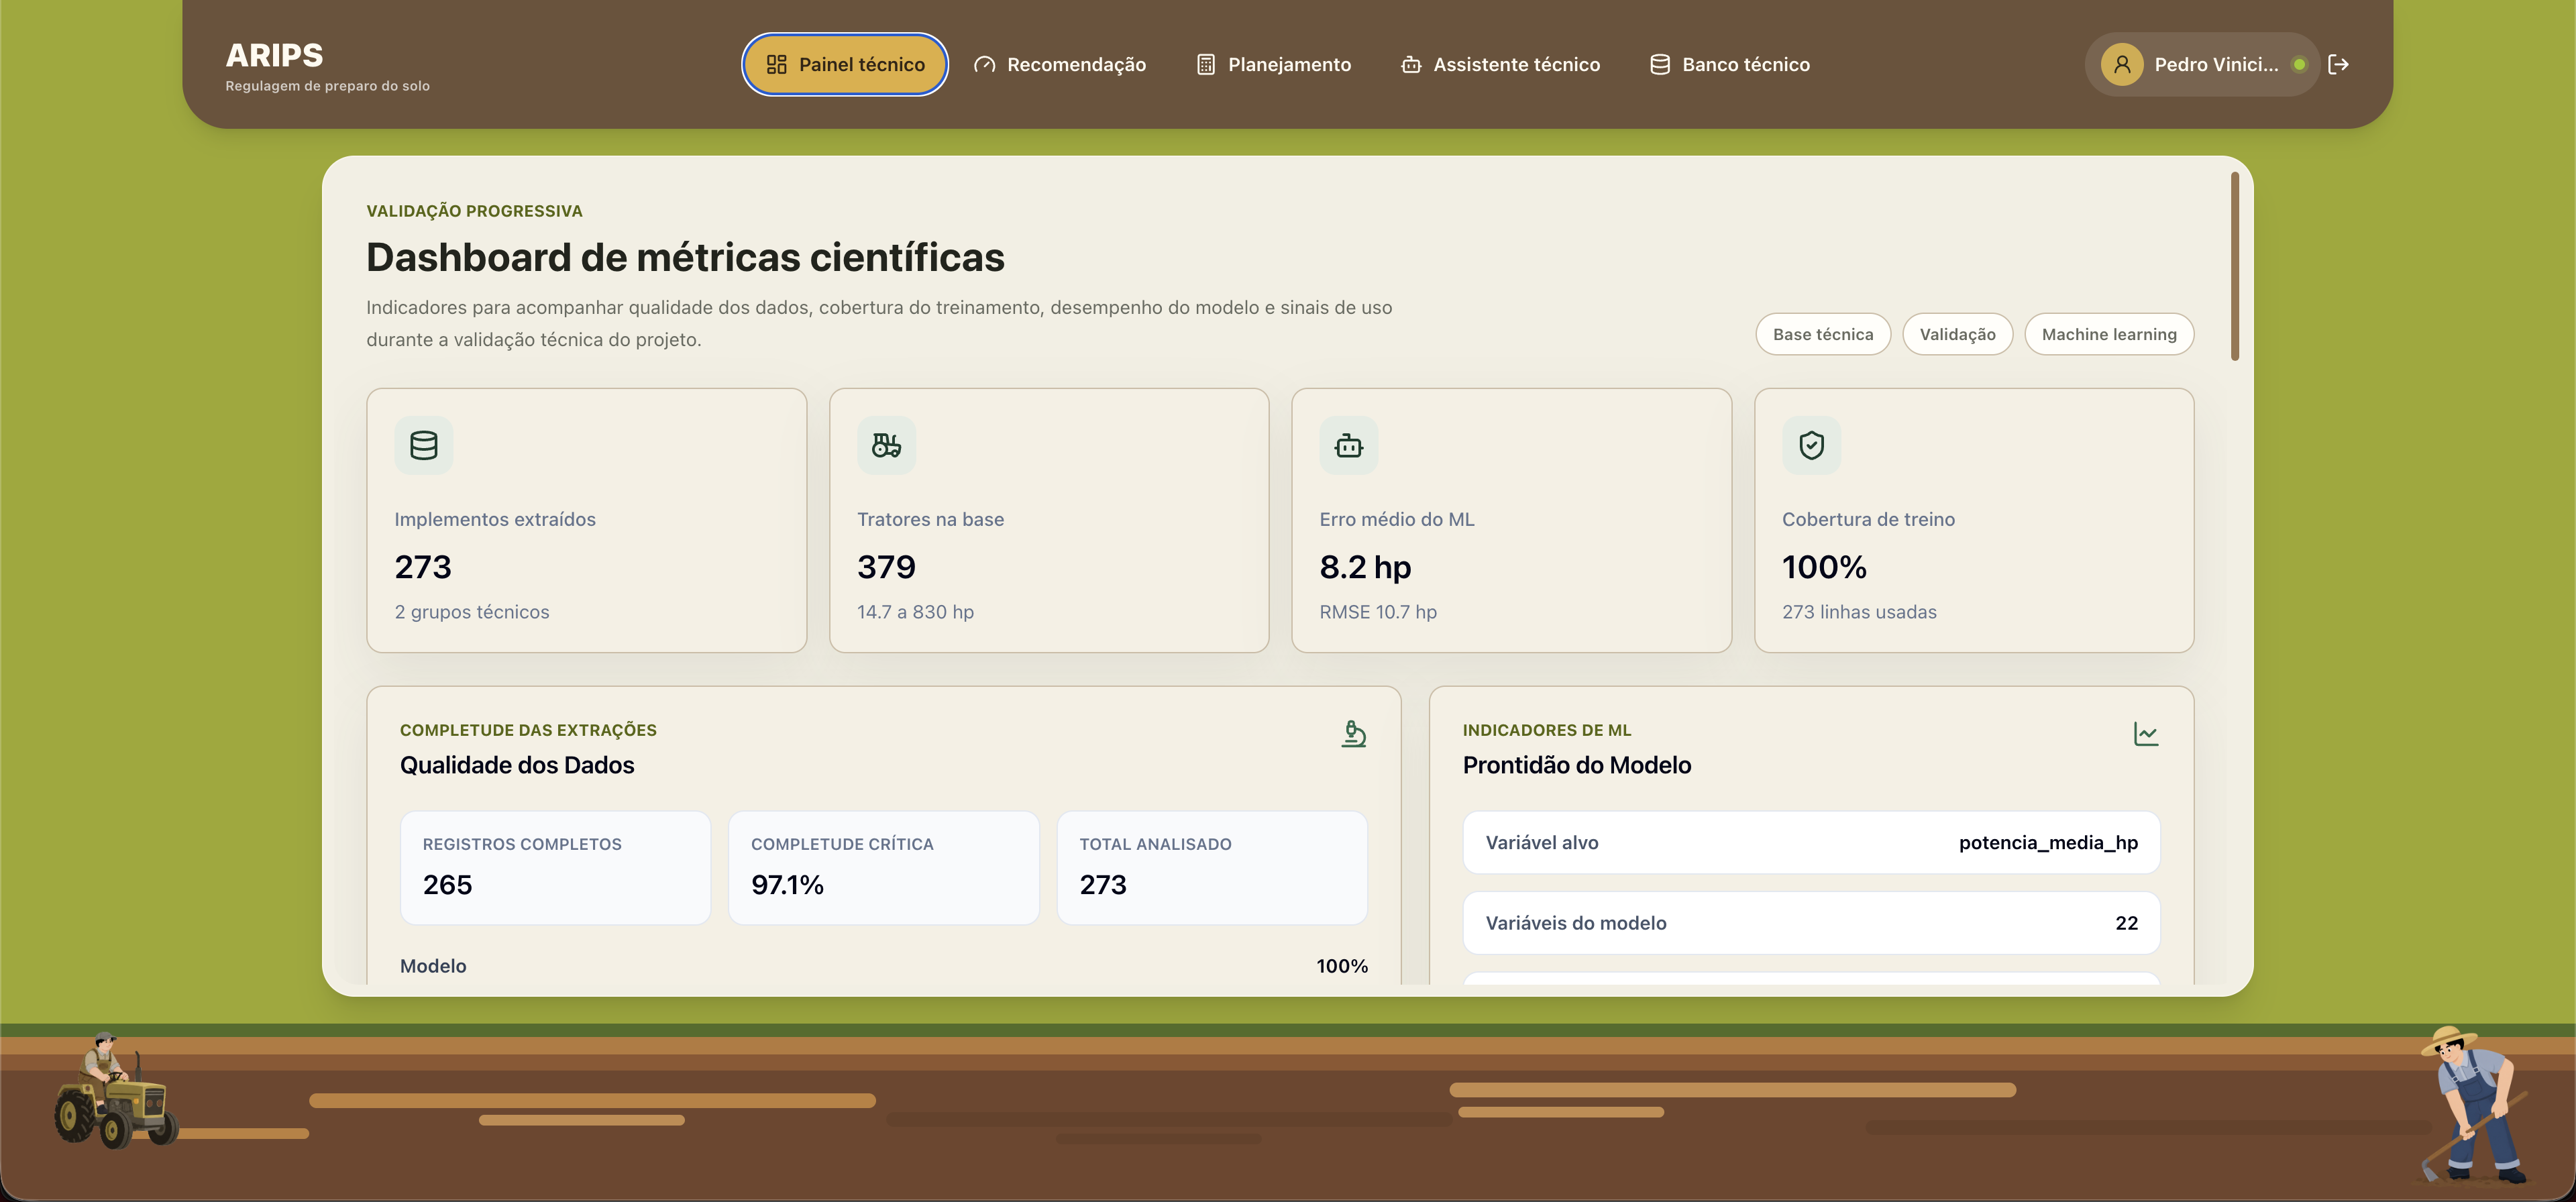
\includegraphics[width=\linewidth]{painel-tecnico.png}
\caption{Painel técnico com indicadores de qualidade da base e desempenho do modelo.}
\label{fig:painel}
\fonteautor
\end{figure}

A Figura~\ref{fig:painel} apresenta o painel administrativo construído para acompanhar a validação progressiva. O painel evita que o modelo seja observado apenas por uma métrica. Ele reúne completude, distribuição de potência, famílias técnicas, disponibilidade de tratores e sinais de uso, permitindo identificar se uma melhoria no erro foi obtida às custas de perda de cobertura ou de concentração excessiva em uma família.

\subsection{Autenticação e experiência inicial}

As telas de entrada e registro foram construídas a partir dos protótipos realizados no Canva. A composição visual relaciona o caminho do campo, a máquina e a paleta da aplicação, enquanto o formulário permanece em uma área de contraste suficiente para leitura. No cadastro, a validação de CPF ocorre antes da persistência, e e-mail e CPF possuem índices únicos.

\begin{figure}[H]
\centering
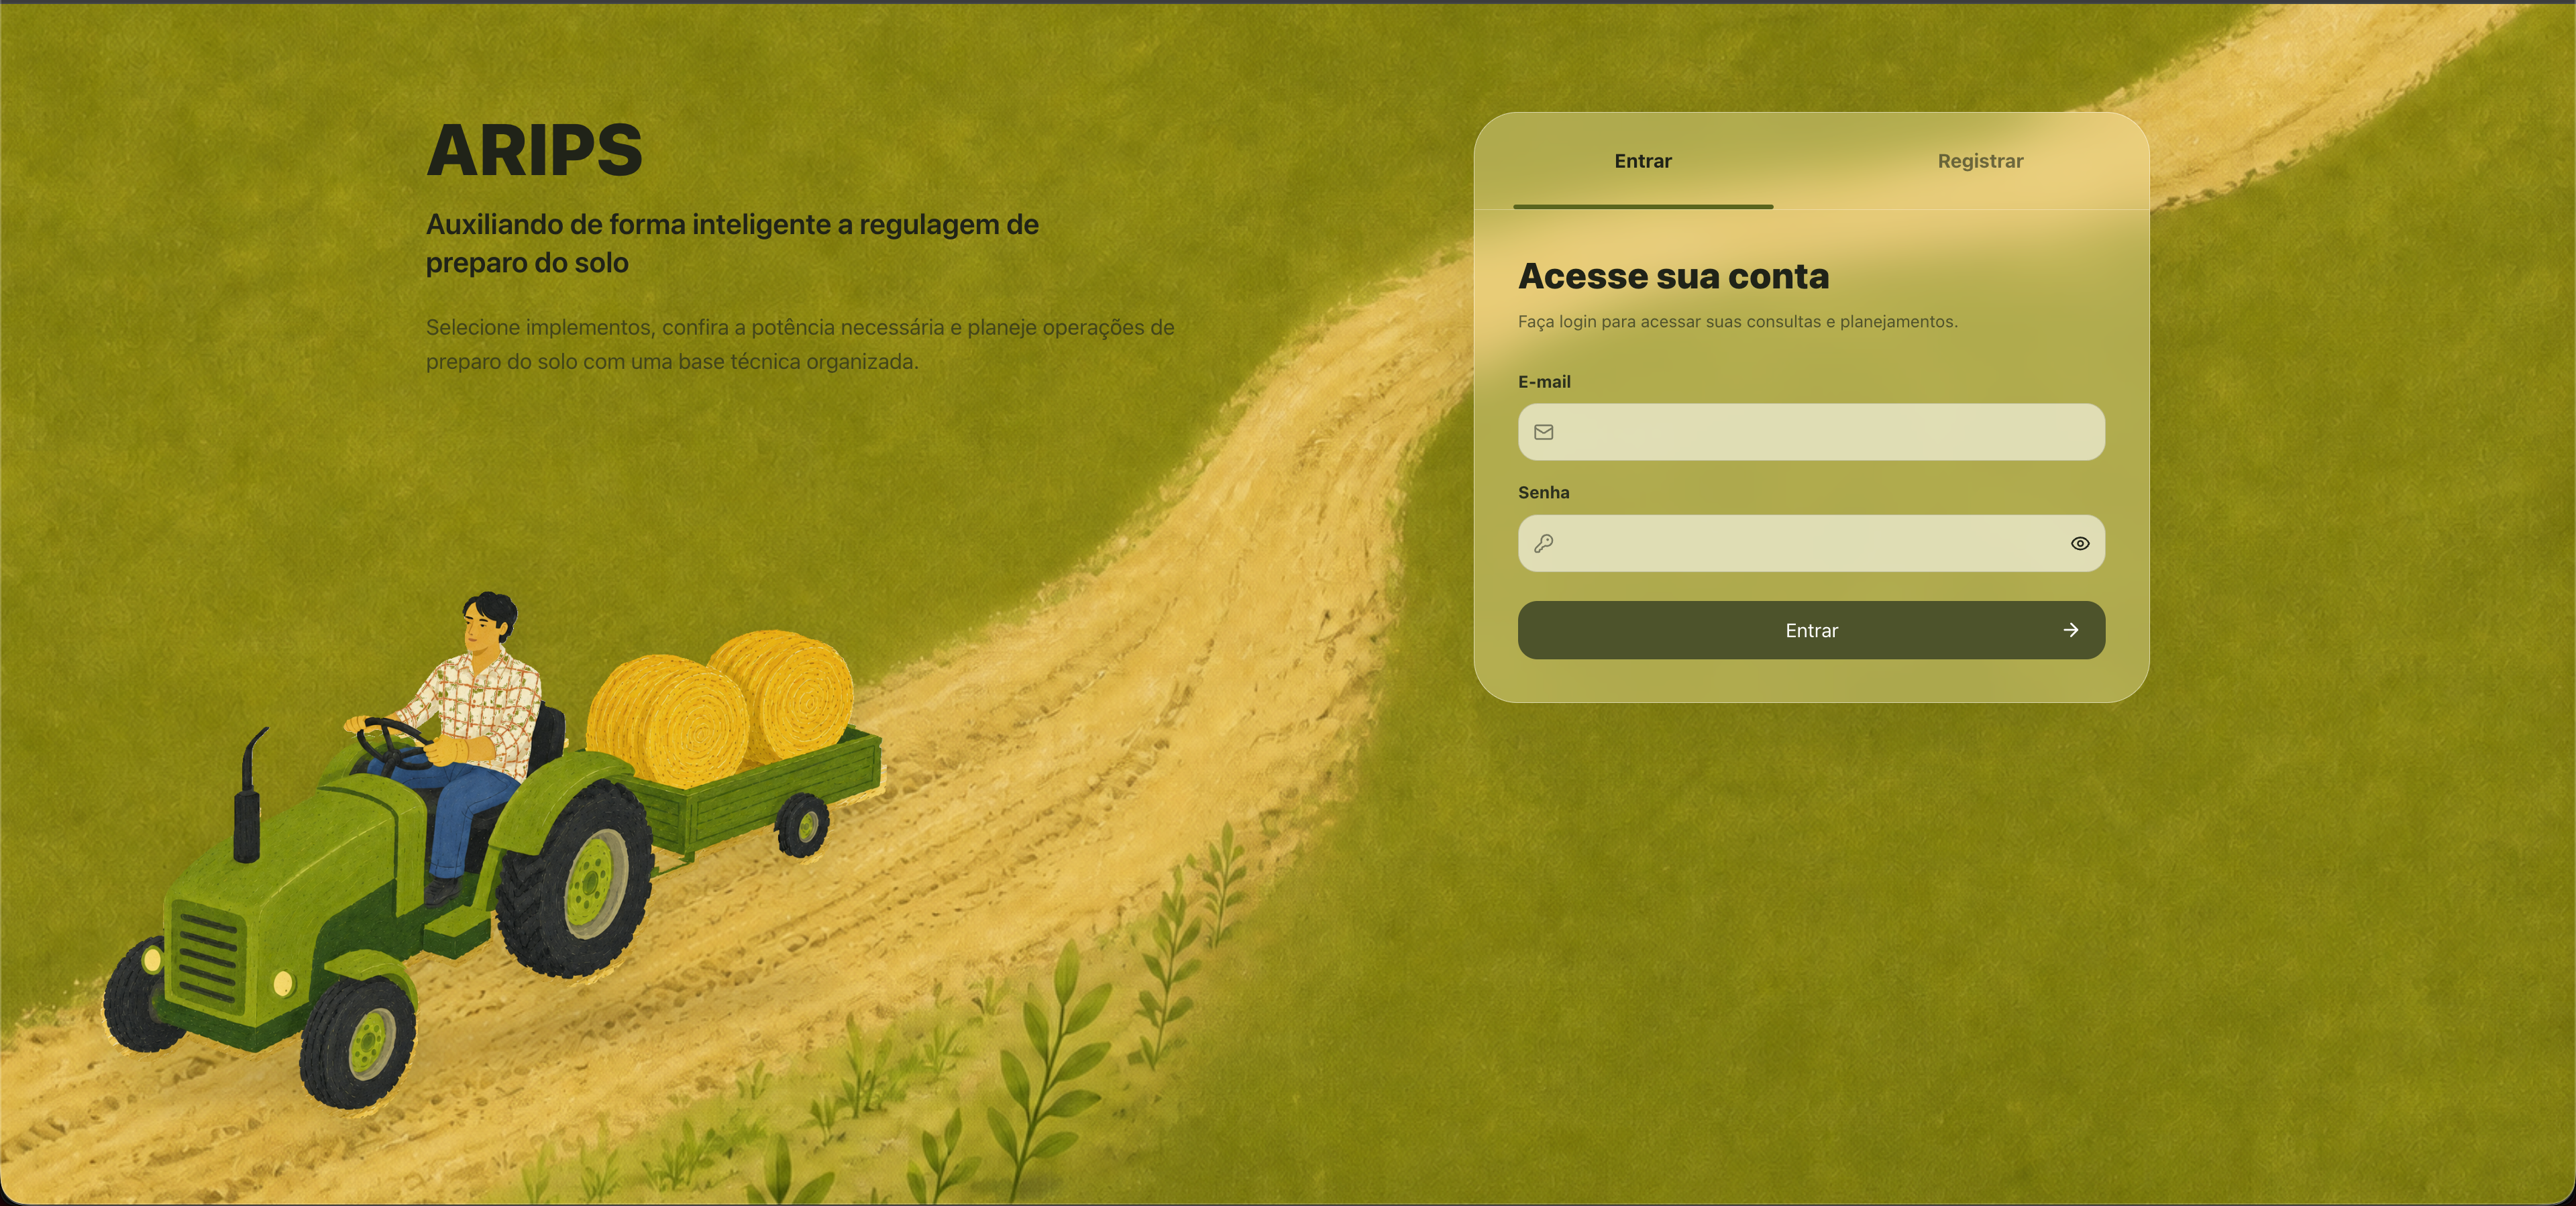
\includegraphics[width=\linewidth]{entrar.png}
\caption{Tela de entrada do ARIPS.}
\label{fig:autenticacao}
\fonteautor
\end{figure}

\begin{figure}[H]
\centering
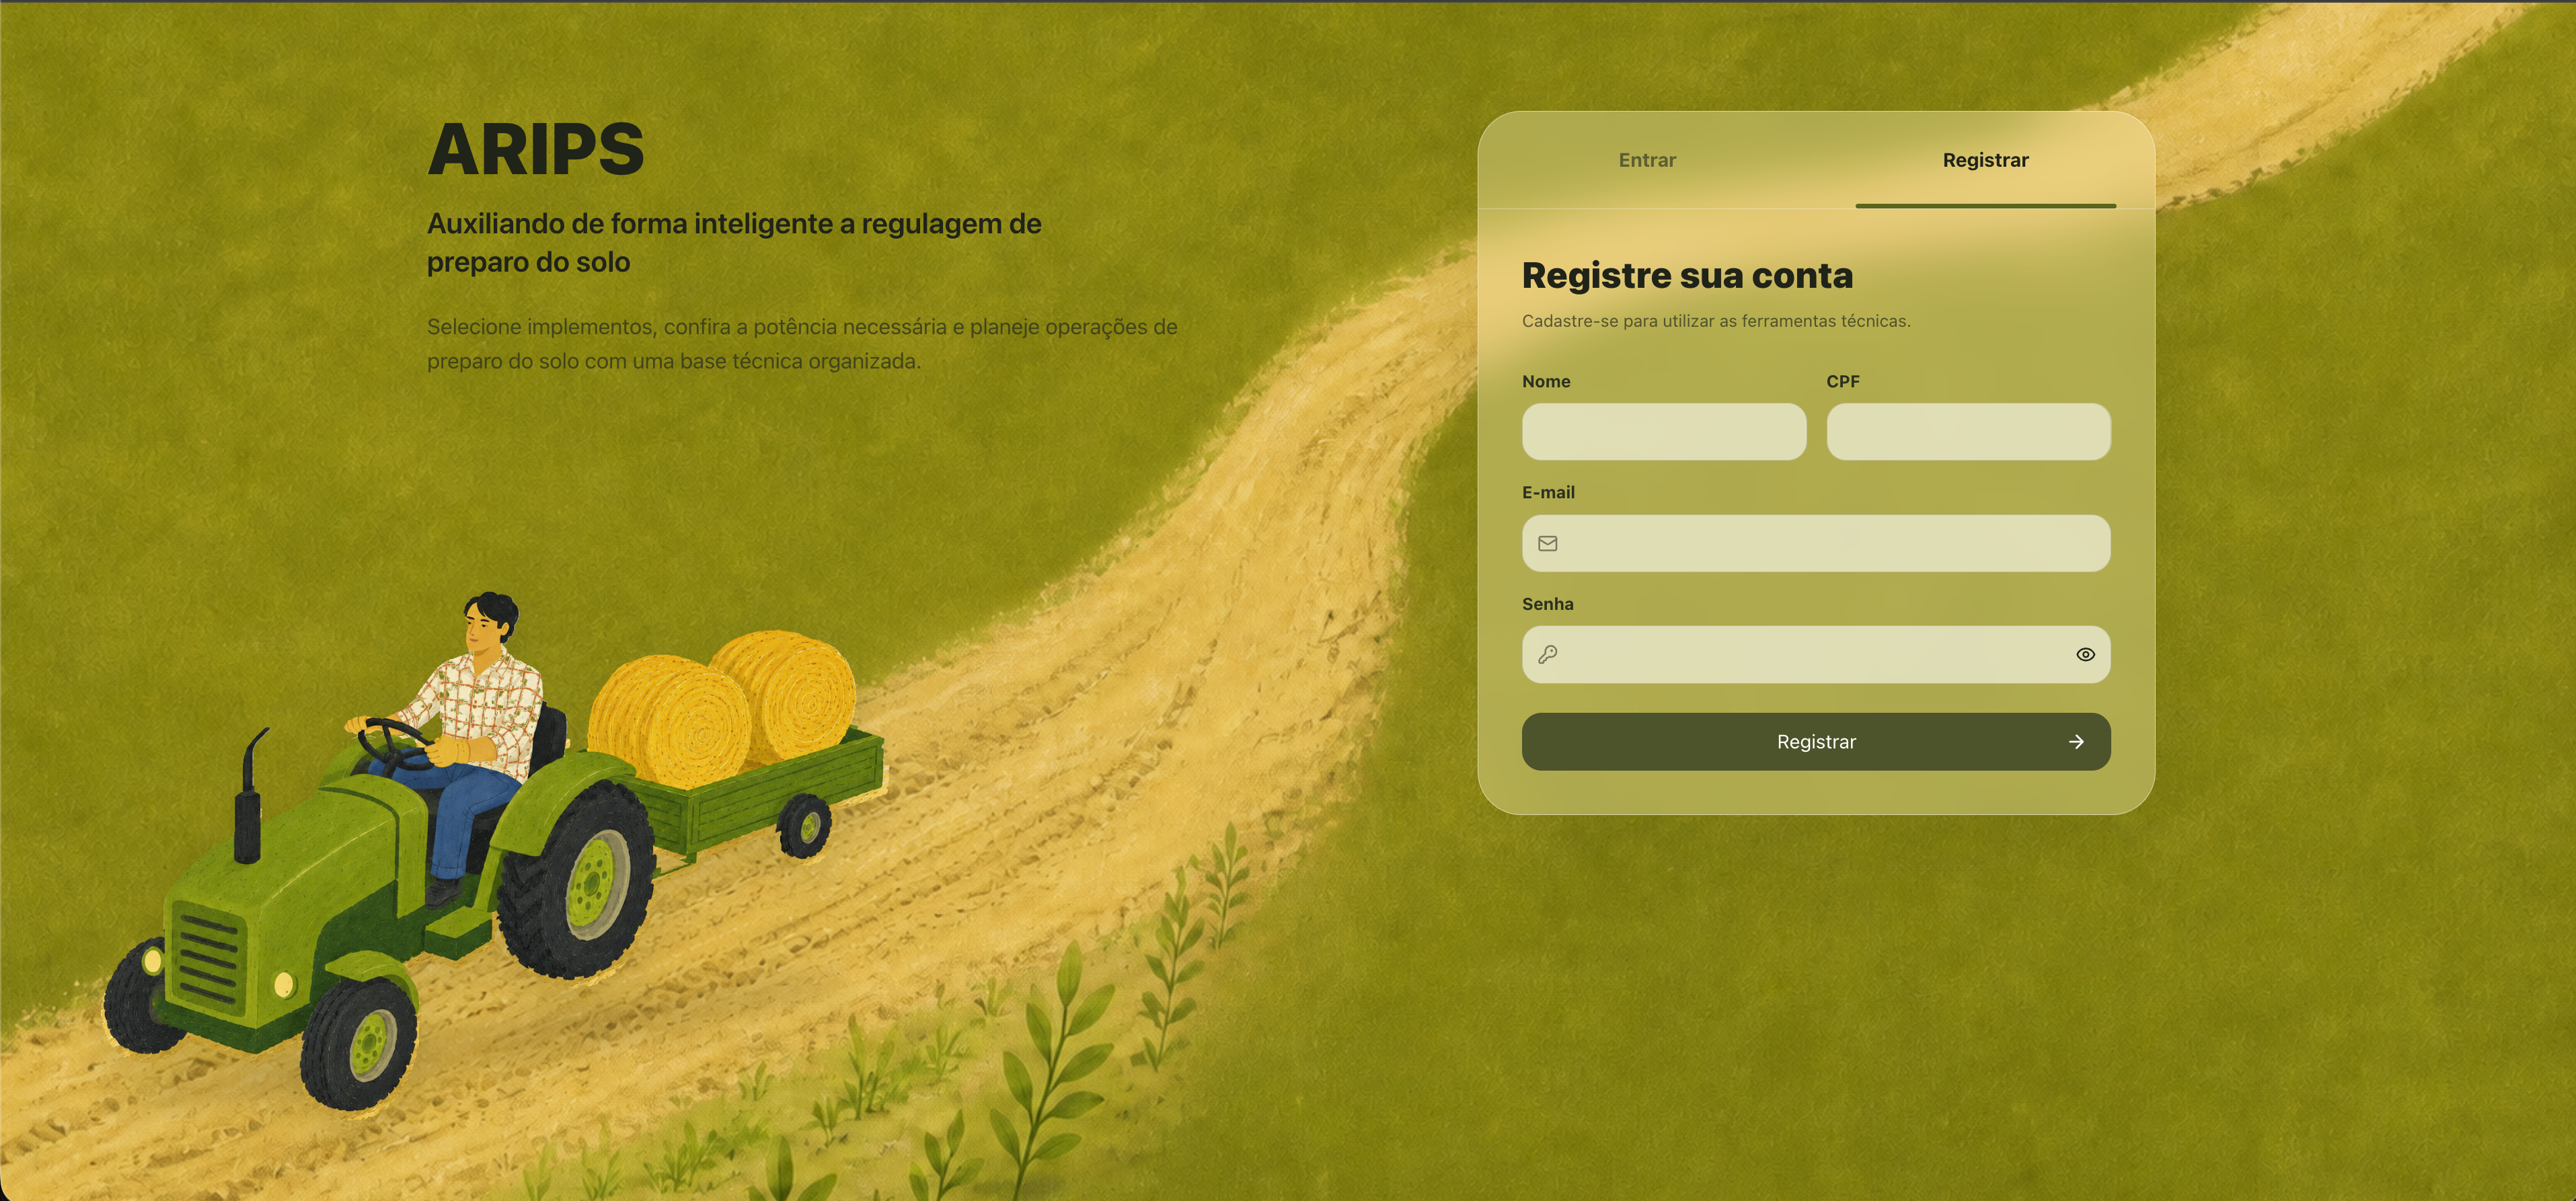
\includegraphics[width=\linewidth]{registrar.png}
\caption{Tela de registro com os campos submetidos à validação da API.}
\label{fig:registro}
\fonteautor
\end{figure}

\subsection{Planejamento de conjuntos mecanizados}

O módulo de planejamento ampliou a proposta inicial porque transforma os dados do banco em uma estimativa operacional. No exemplo da Figura~\ref{fig:planejamento}, uma área de 120 ha e um período de 128 dias resultaram em 1024 horas disponíveis. O sistema distribuiu 682,67 horas para aração e 341,33 horas para gradagens, calculando em seguida a largura e a quantidade de conjuntos para cada operação.

\begin{figure}[H]
\centering
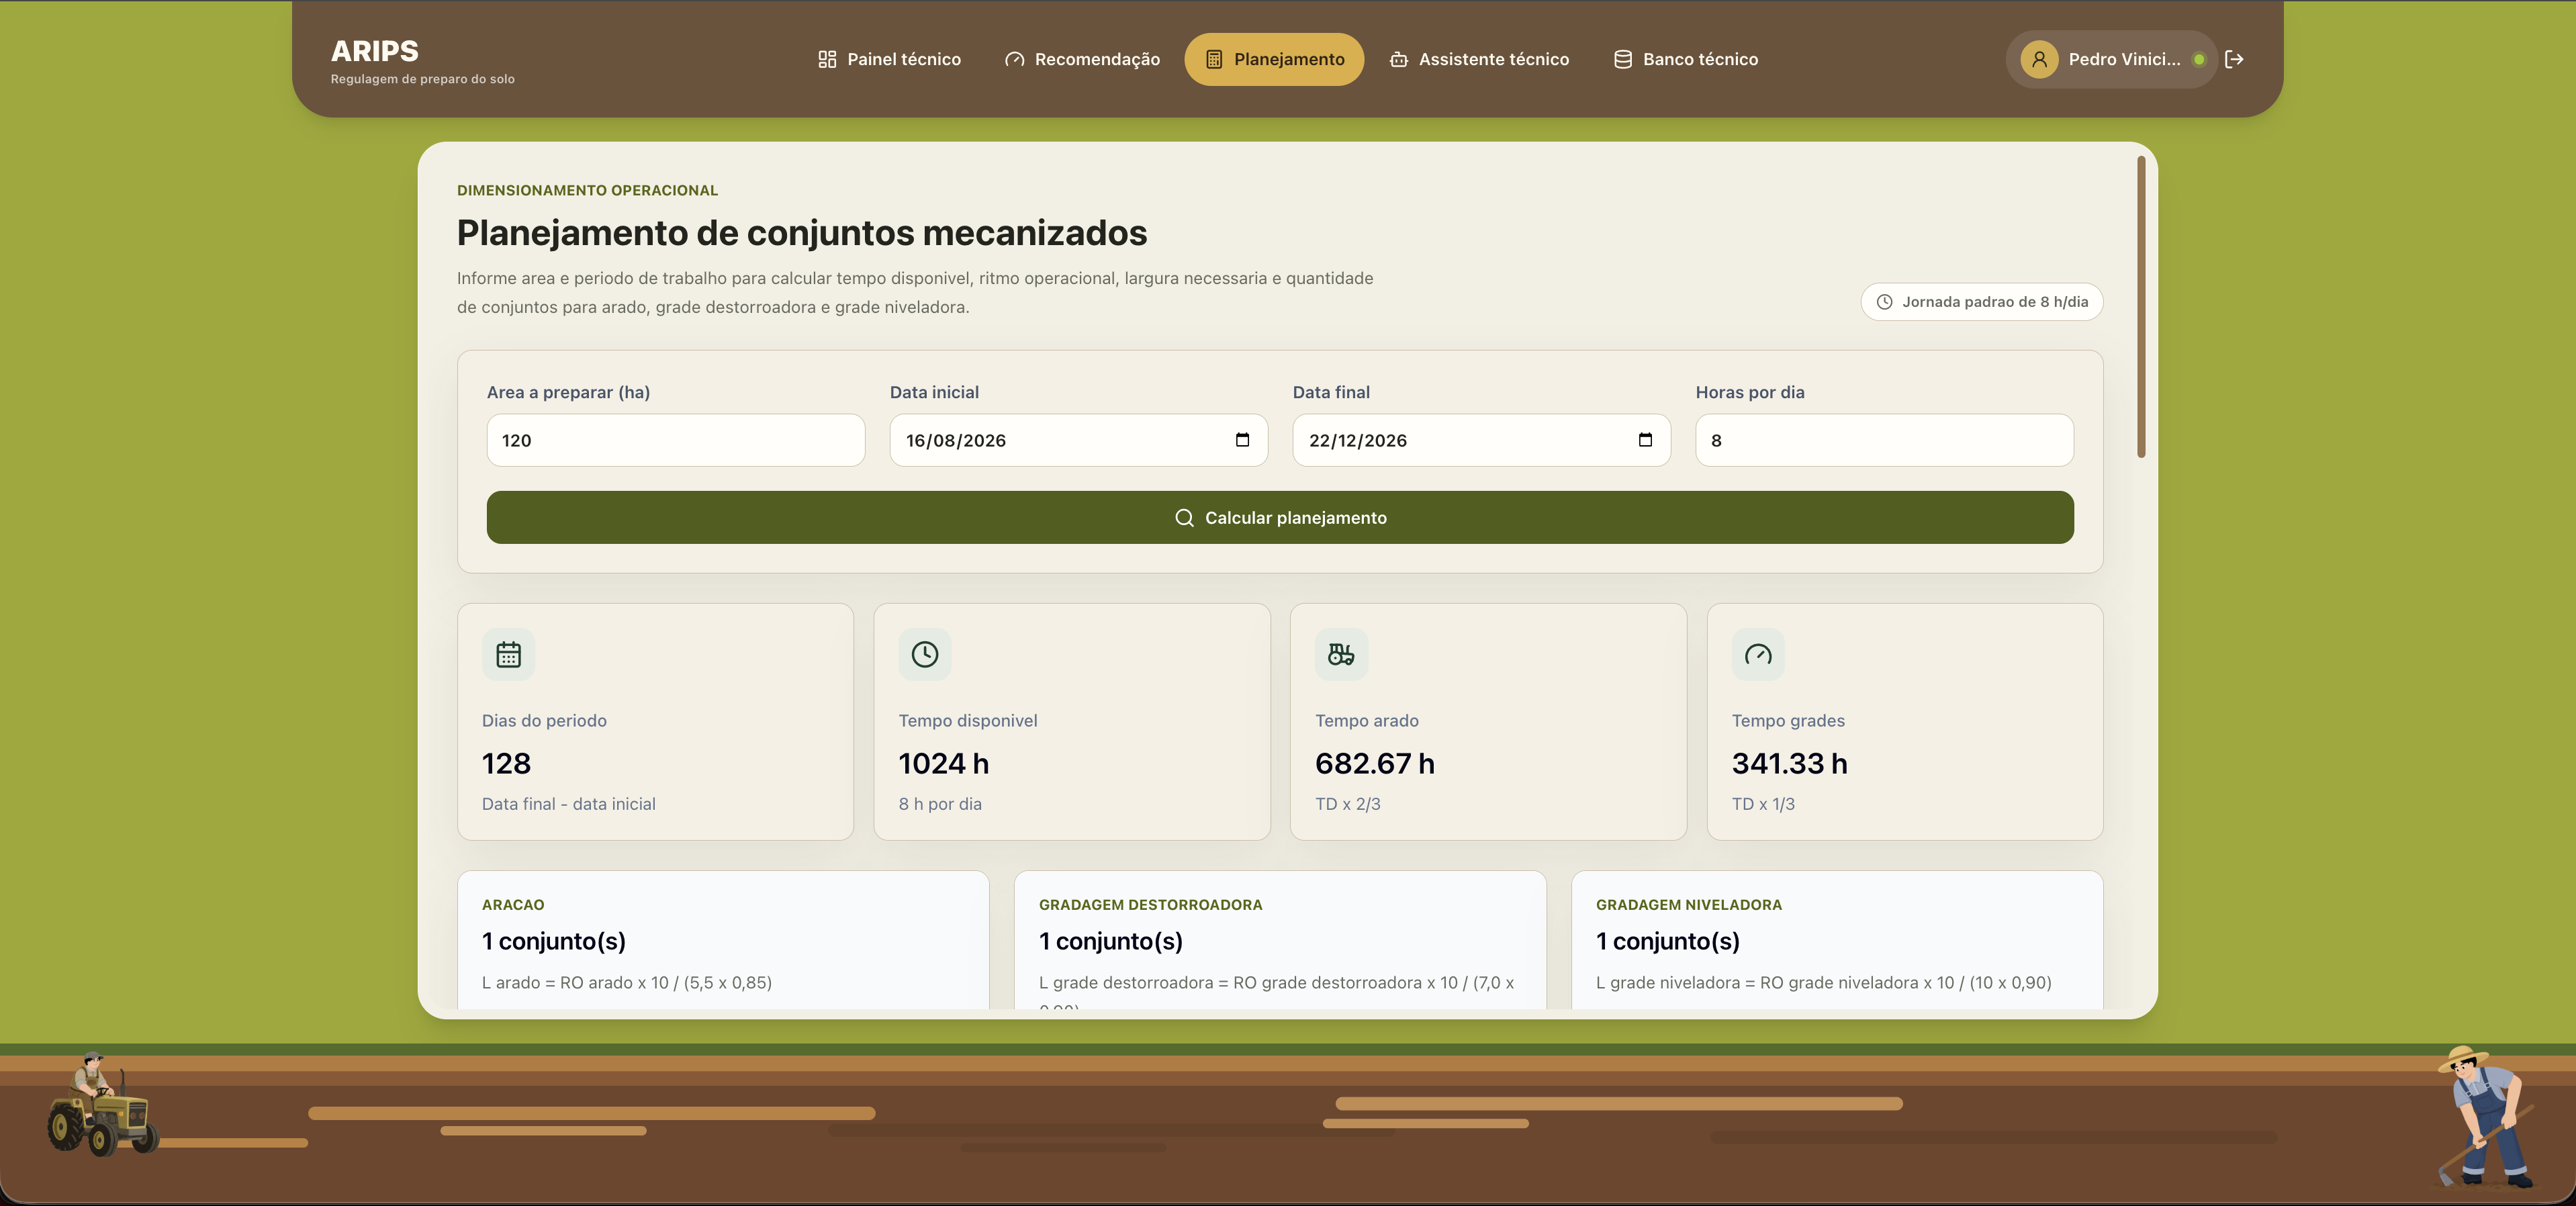
\includegraphics[width=\linewidth]{planejamento.png}
\caption{Tela de planejamento operacional com distribuição do tempo e dimensionamento dos conjuntos.}
\label{fig:planejamento}
\fonteautor
\end{figure}

Esse resultado aproxima a aplicação de uma ferramenta de apoio à decisão, mas deve ser interpretado como pré-dimensionamento. A eficiência de campo e a velocidade são valores de referência fixados no serviço, enquanto relevo, formato do talhão, manobras, paradas e condição superficial podem alterar a capacidade efetiva. A utilidade principal é mostrar rapidamente se o período disponível é compatível com a área e quais características mínimas devem ser procuradas.

\subsection{Assistente técnico e respostas controladas}

A interface do assistente foi organizada com histórico, sugestões de perguntas, área de mensagens e caixa de entrada fixa. A primeira resposta orienta o usuário a informar potência, solo e operação. A Figura~\ref{fig:assistente} mostra o estado inicial, enquanto a Figura~\ref{fig:resposta} apresenta uma consulta que contém potência, tipo de implemento e textura do solo.

\begin{figure}[H]
\centering
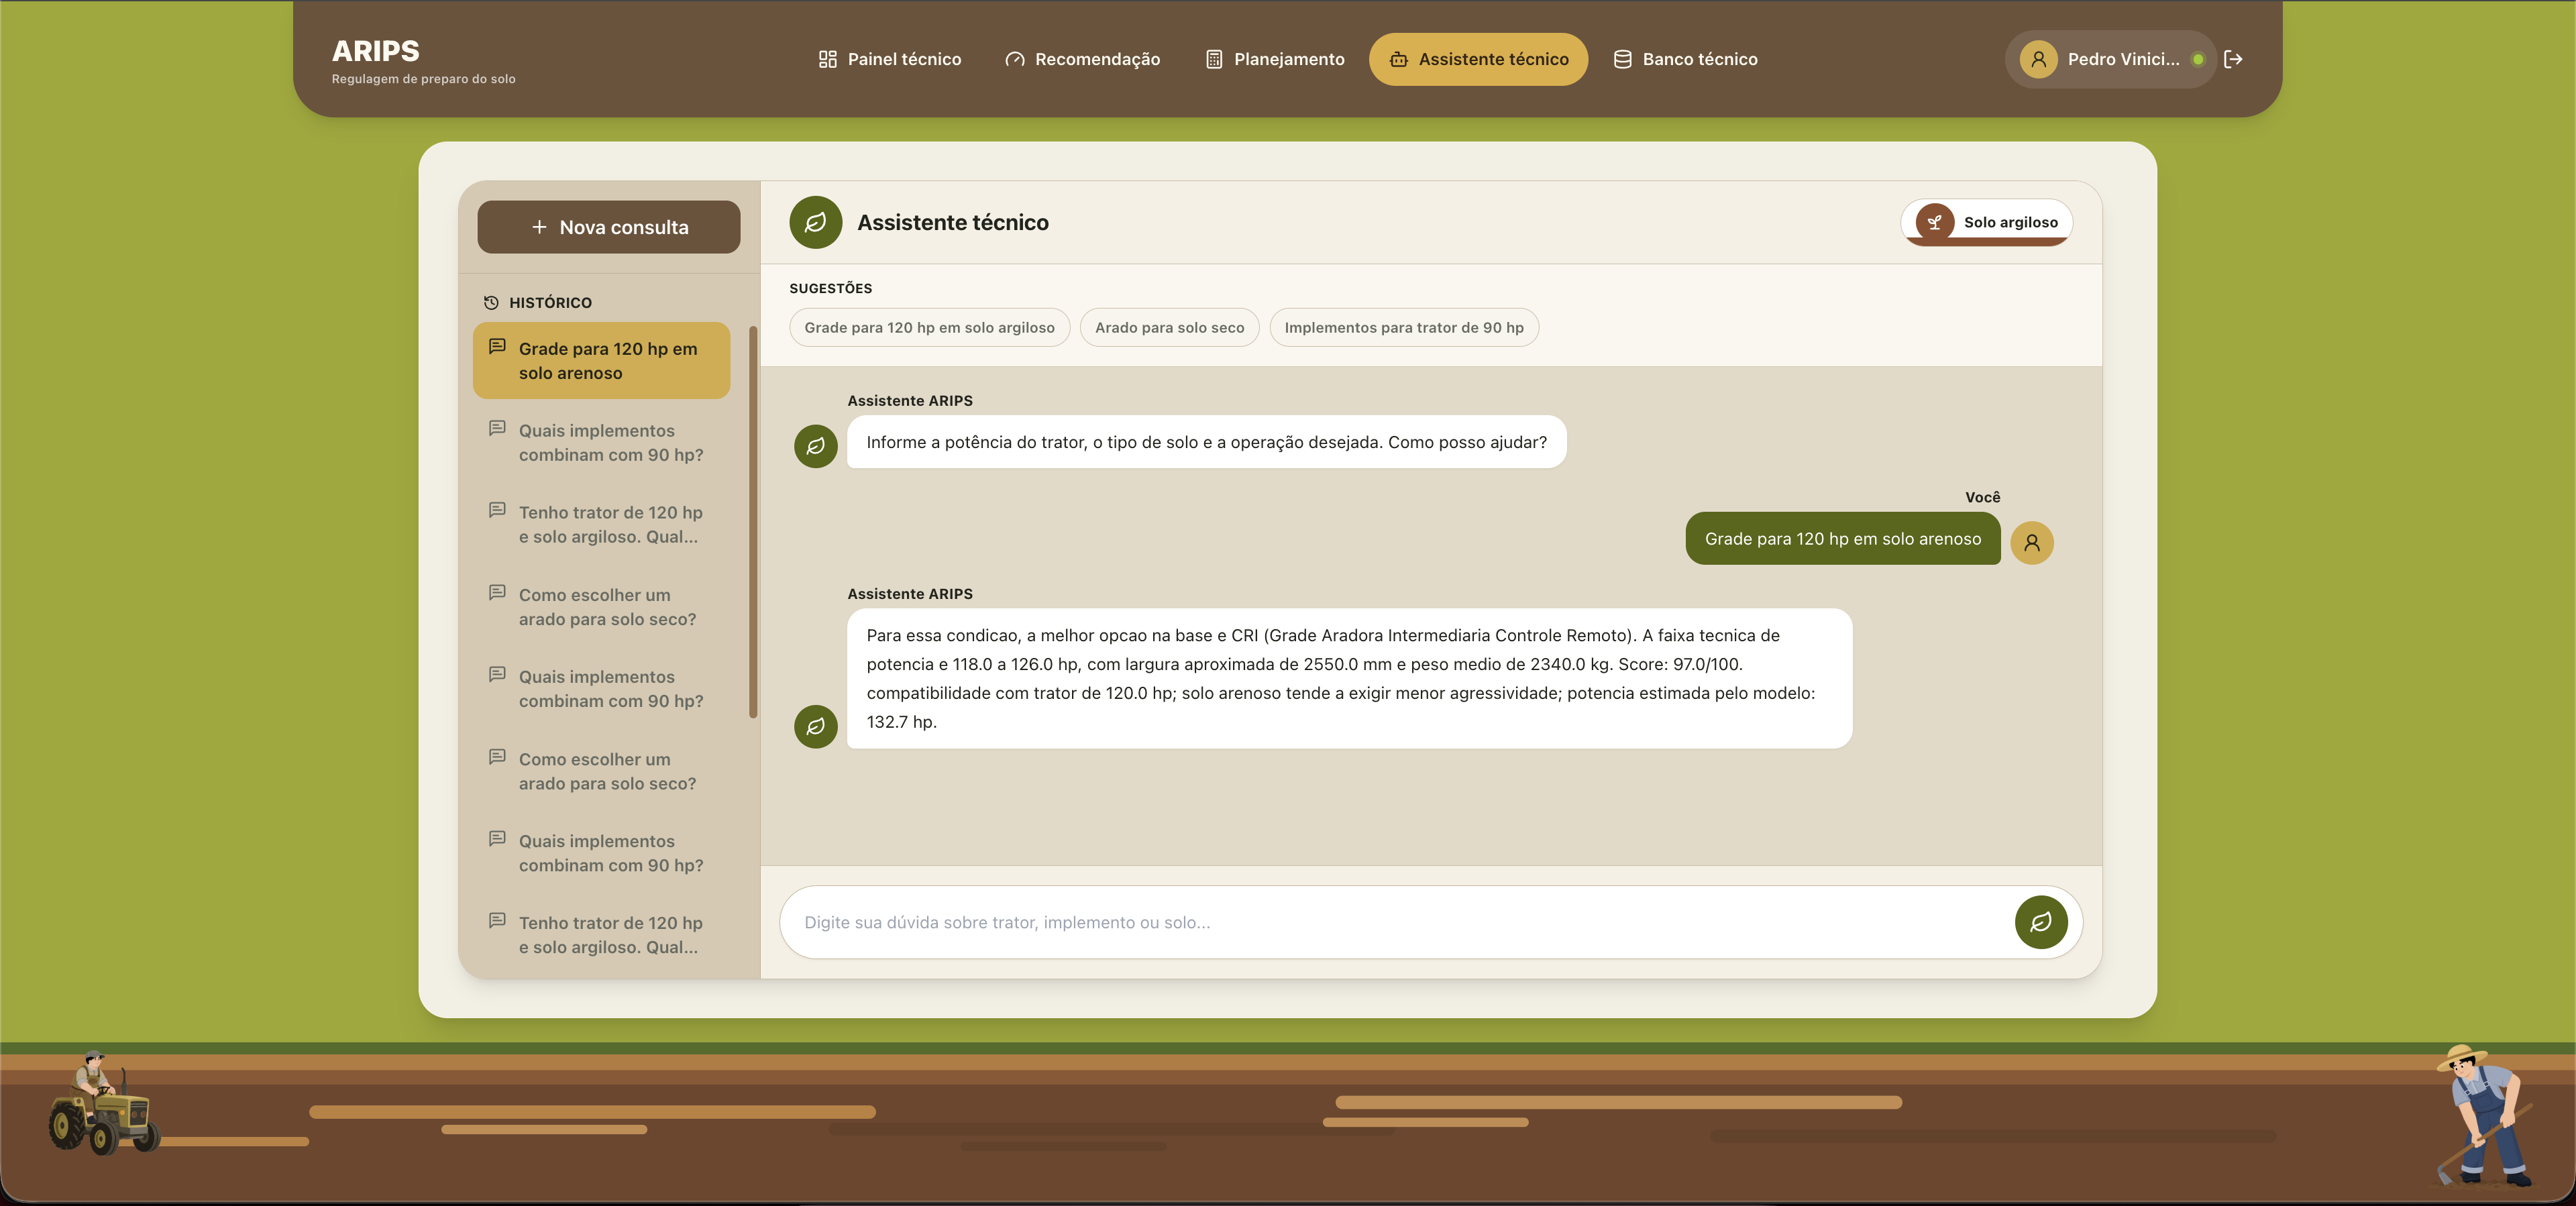
\includegraphics[width=\linewidth]{assistente-tecnico.png}
\caption{Assistente técnico com histórico e sugestões de consultas.}
\label{fig:assistente}
\fonteautor
\end{figure}

\begin{figure}[H]
\centering
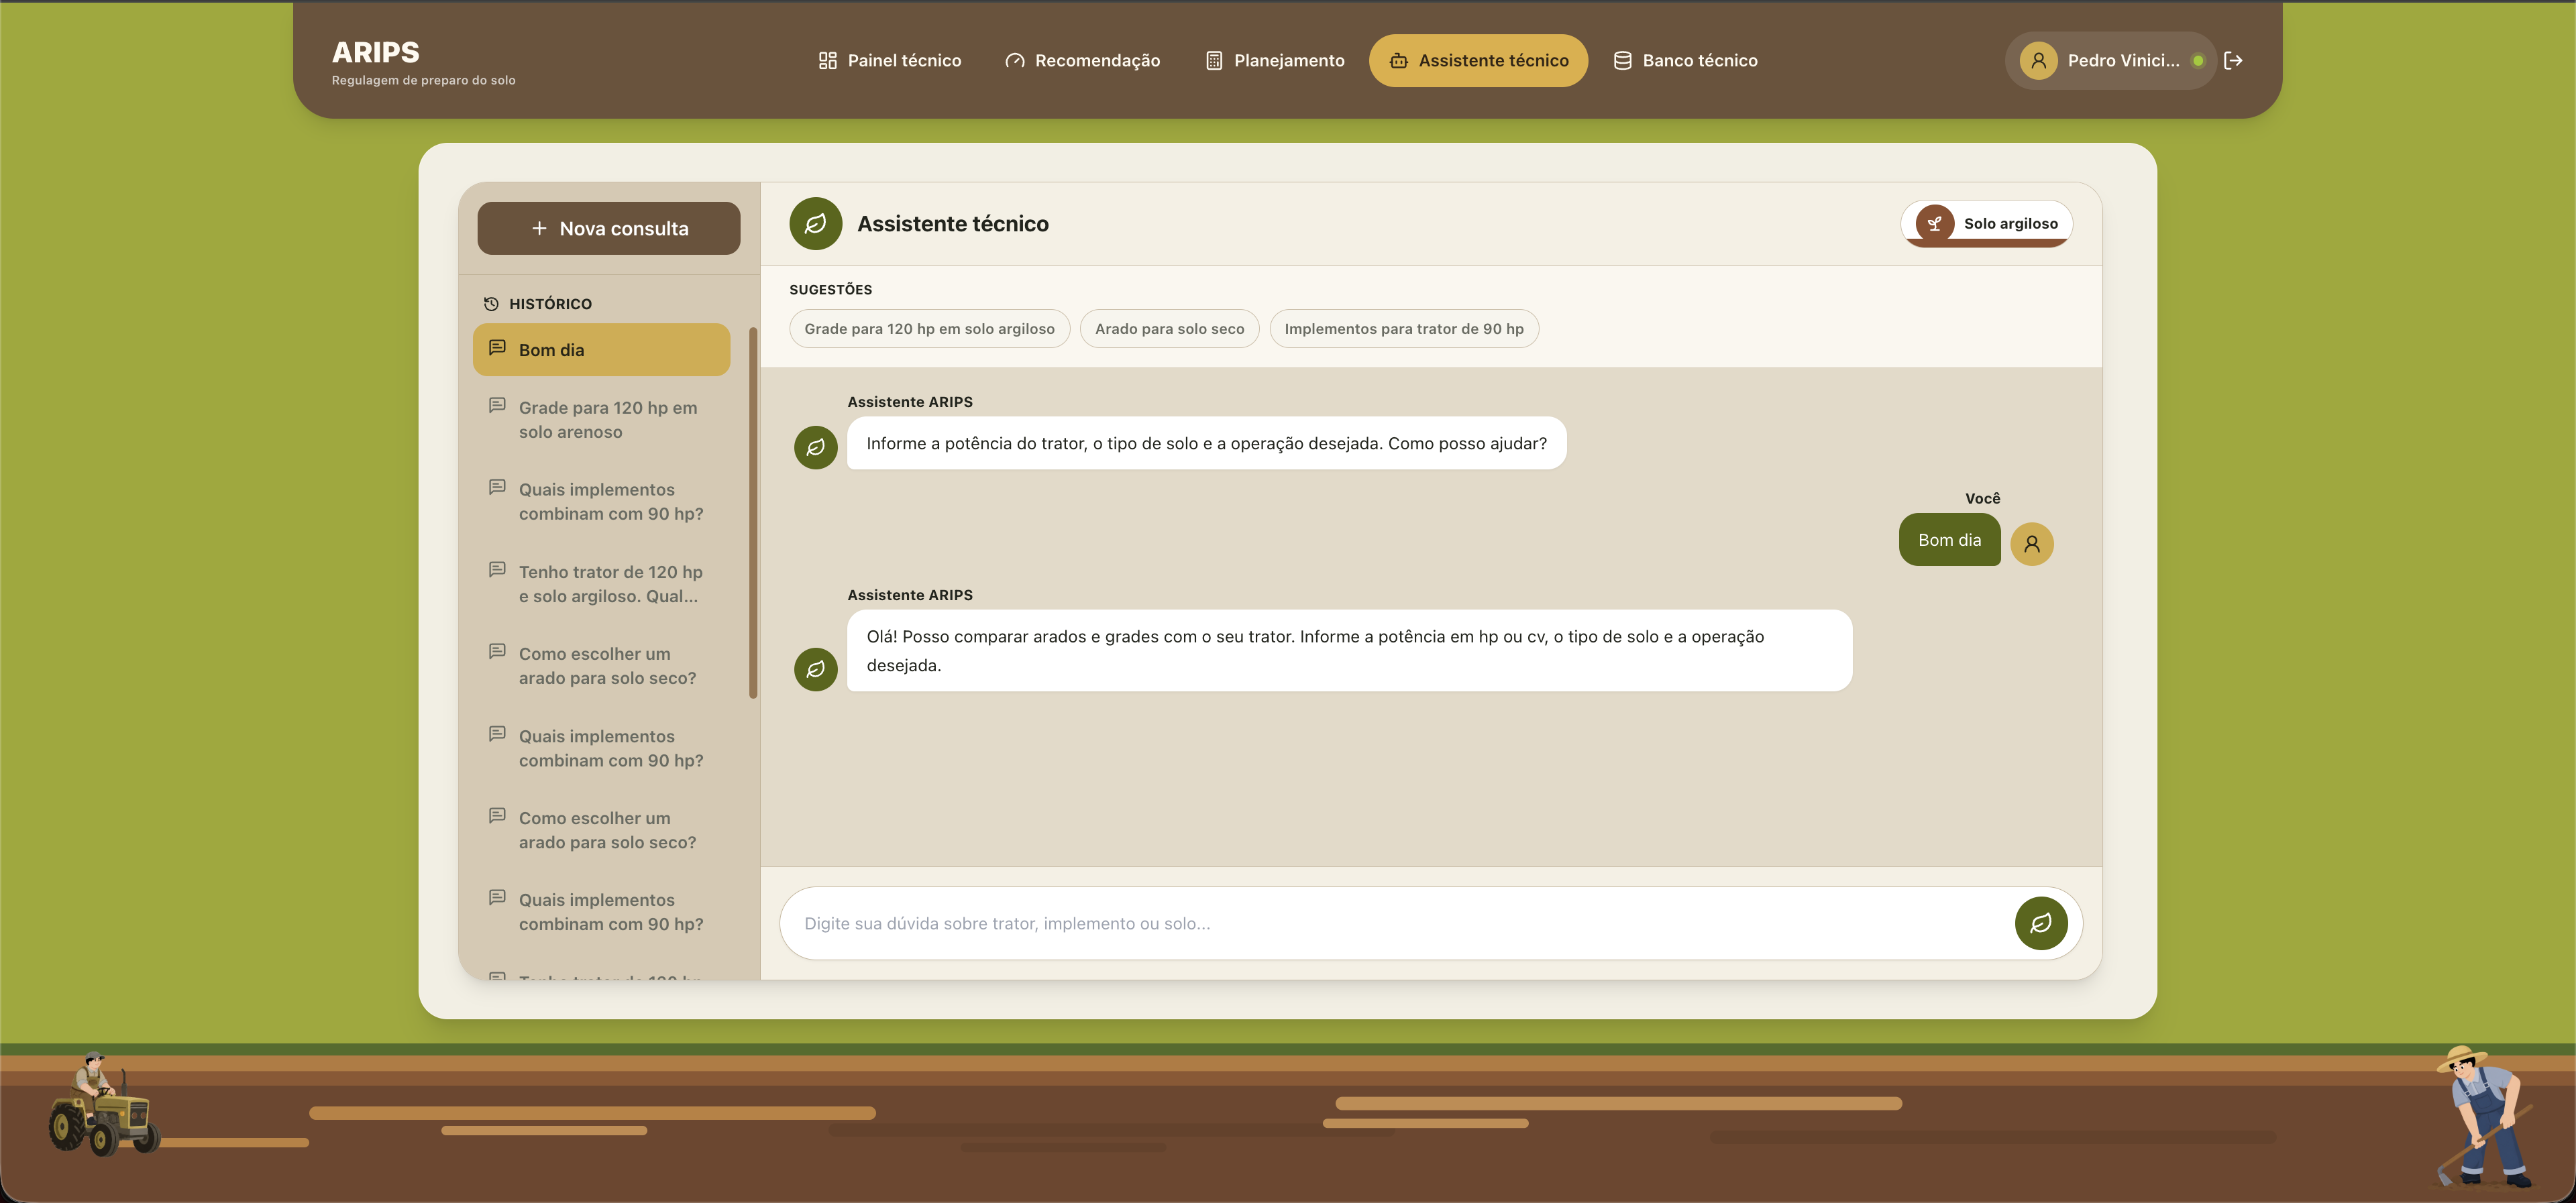
\includegraphics[width=\linewidth]{chatbot-configurado-respostas.png}
\caption{Exemplo de resposta de saudação após a separação das intenções do chatbot.}
\label{fig:resposta}
\fonteautor
\end{figure}

Além da saudação mostrada, o fluxo técnico testado reconheceu perguntas como ``grade para 120 hp em solo arenoso''. Para esse tipo de mensagem, o sistema extrai a potência, identifica o grupo, consulta a base, aplica o modelo e filtra pela faixa declarada. A resposta apresenta até três opções e encerra com a orientação de conferir o manual e realizar uma passagem de teste. O ganho mais importante foi reduzir respostas genéricas e tornar explícito quais dados faltam quando a consulta é insuficiente.

\subsection{Discussão integrada dos resultados}

Os resultados mostram que a decomposição do problema favoreceu a implementação. O OCR pôde ser melhorado sem alterar a interface; o modelo pôde ser treinado novamente sem redesenhar o banco; e o chatbot pôde receber filtros adicionais sem mudar o processo de extração. Essa independência relativa confirma a utilidade da arquitetura modular e do SRP.

Ao mesmo tempo, o pensamento complexo ajuda a reconhecer que a soma das partes não garante uma recomendação agronômica completa. A potência adequada depende de fatores que os catálogos não registram de forma uniforme, e a textura do solo, a umidade e a profundidade ainda entram como regras. A aplicação produz uma orientação baseada na melhor informação disponível, mas a interpretação precisa continuar ligada ao contexto e à experiência de campo.

Também houve uma diferença importante em relação ao plano inicial. Em vez de iniciar por um modelo de linguagem ou por uma floresta aleatória, foi priorizada a qualidade do dado, a rastreabilidade e a construção de uma aplicação funcional. Essa decisão reduziu a complexidade prematura e tornou visíveis as lacunas da base. A solução final é mais restrita, porém suas respostas podem ser relacionadas aos registros utilizados e às regras implementadas.

\section{Conclusões}

O projeto alcançou o objetivo de construir uma aplicação web integrada para apoio à regulagem e ao planejamento de implementos de preparo do solo. A principal contribuição foi transformar documentos técnicos dispersos em uma base consultável, com 273 configurações de implementos e 379 tratores, e utilizar essa base em diferentes funções: painel, pesquisa, recomendação, planejamento e chatbot.

O uso conjunto de PyMuPDF, OCR, regras de extração e revisão permitiu superar parte das dificuldades dos PDFs. O modelo Ridge produziu MAE de 8,19 hp e RMSE de 10,70 hp nas linhas de treinamento, mantendo um artefato simples e auditável. O mecanismo híbrido, ao preservar as faixas declaradas e aplicar um filtro final de compatibilidade, mostrou-se mais adequado à etapa atual do que uma decisão inteiramente dependente do modelo.

O desenvolvimento do backend, da autenticação, do tratamento tipado de erros e da interface resultou em um sistema utilizável por administradores e usuários comuns. O chatbot passou a diferenciar saudações, orientações, recomendações e pedidos de esclarecimento, além de manter histórico por usuário. Os testes automatizados também estabeleceram uma base para alterações futuras.

Por fim, o trabalho evidenciou que o pensamento computacional e o pensamento complexo não são contraditórios. A decomposição tornou o problema implementável, enquanto a recomposição das relações impediu que uma métrica isolada fosse confundida com validação agronômica. O ARIPS deve ser considerado um protótipo técnico funcional em validação computacional, preparado para receber dados e avaliações de campo.

\section{Perspectivas de futuros trabalhos}

\begin{sloppypar}
Como continuidade, a primeira necessidade é realizar validação externa. Recomenda-se separar dados de treino e teste, aplicar validação cruzada por família e coletar exemplos que não tenham participado da construção da base. Depois, a regressão Ridge, a floresta aleatória e métodos de árvores impulsionadas poderão ser comparados com o mesmo protocolo, observando não apenas MAE e RMSE, mas também erro por faixa de potência, estabilidade entre famílias e calibração do ranking.
\end{sloppypar}

Também devem ser coletadas medições de campo: velocidade real, patinagem, consumo de combustível, profundidade obtida, umidade, textura, resistência à penetração e avaliação da qualidade do preparo. Esses dados permitiriam treinar modelos associados ao desempenho operacional, e não apenas à potência média de catálogo. Uma etapa de validação com engenheiros agrícolas, agrônomos e operadores deve classificar as recomendações quanto à segurança, clareza e utilidade.

No chatbot, a continuidade inclui ampliar o corpus de perguntas reais, reconhecer variações regionais da linguagem e implementar recuperação de trechos dos manuais com indicação da fonte. Uma arquitetura de geração aumentada por recuperação pode ser estudada, desde que as respostas permaneçam restritas à base e apresentem evidência verificável. Também é possível integrar sensores de umidade e compactação, mantendo a entrada manual como alternativa para propriedades sem conectividade.

Por fim, a cobertura de testes deve ser ampliada para os repositórios, o treinamento e os principais fluxos do frontend. Testes ponta a ponta, avaliação de acessibilidade, registro de versões do conjunto de dados e monitoramento das recomendações completarão a infraestrutura necessária para uma implantação controlada em propriedades parceiras.

\section{Referências bibliográficas}

\sloppy
\begin{thebibliography}{99}

\bibitem{embrapa_melancia}
EMBRAPA. \textbf{Solos: preparo do solo}. Sistema de Produção de Melancia. Brasília, DF: Empresa Brasileira de Pesquisa Agropecuária, 2010. Disponível em: \url{https://sistemasdeproducao.cnptia.embrapa.br/FontesHTML/Melancia/SistemaProducaoMelancia/solos.htm}. Acesso em: 19 ago. 2026.

\bibitem{embrapa_feijao}
EMBRAPA. \textbf{Preparo do solo}. Agência de Informação Tecnológica: Feijão. Brasília, DF: Empresa Brasileira de Pesquisa Agropecuária, 2021. Disponível em: \url{https://portaldxp-h.sede.embrapa.br/en/web/agencia-de-informacao-tecnologica/cultivos/feijao/producao/preparo-do-solo}. Acesso em: 19 ago. 2026.

\bibitem{ibge2019}
IBGE. \textbf{Censo Agro 2017: população ocupada nos estabelecimentos agropecuários cai 8,8\%}. Agência de Notícias, 25 out. 2019. Disponível em: \url{https://agenciadenoticias.ibge.gov.br/agencia-sala-de-imprensa/2013-agencia-de-noticias/releases/25789-censo-agro-2017-populacao-ocupada-nos-estabelecimentos-agropecuarios-cai-8-8}. Acesso em: 19 ago. 2026.

\bibitem{ibge2017}
IBGE. \textbf{Censo Agropecuário 2017: resultados definitivos}. Rio de Janeiro: IBGE, 2019. Disponível em: \url{https://biblioteca.ibge.gov.br/visualizacao/periodicos/3096/agro_2017_resultados_definitivos.pdf}. Acesso em: 19 ago. 2026.

\bibitem{morin2000}
MORIN, Edgar. \textbf{Os sete saberes necessários à educação do futuro}. 2. ed. São Paulo: Cortez; Brasília, DF: UNESCO, 2000.

\bibitem{morin2015}
MORIN, Edgar. \textbf{Introdução ao pensamento complexo}. 5. ed. Porto Alegre: Sulina, 2015.

\bibitem{wing2006}
WING, Jeannette M. Computational thinking. \textbf{Communications of the ACM}, New York, v. 49, n. 3, p. 33--35, 2006. DOI: \url{https://doi.org/10.1145/1118178.1118215}.

\bibitem{pymupdf_text}
ARTIFEX. \textbf{PyMuPDF documentation: details on text extraction}. 2026. Disponível em: \url{https://pymupdf.readthedocs.io/en/latest/app1.html}. Acesso em: 19 ago. 2026.

\bibitem{pymupdf_ocr}
ARTIFEX. \textbf{PyMuPDF documentation: optical character recognition}. 2026. Disponível em: \url{https://pymupdf.readthedocs.io/en/latest/recipes-ocr.html}. Acesso em: 19 ago. 2026.

\bibitem{hoerl1970}
HOERL, Arthur E.; KENNARD, Robert W. Ridge regression: biased estimation for nonorthogonal problems. \textbf{Technometrics}, v. 12, n. 1, p. 55--67, 1970. DOI: \url{https://doi.org/10.1080/00401706.1970.10488634}.

\bibitem{hastie2009}
HASTIE, Trevor; TIBSHIRANI, Robert; FRIEDMAN, Jerome. \textbf{The elements of statistical learning}. 2. ed. New York: Springer, 2009.

\bibitem{martin2003}
MARTIN, Robert C. \textbf{Agile software development: principles, patterns, and practices}. Upper Saddle River: Prentice Hall, 2003.

\bibitem{repositorioarips}
PEREIRA, Pedro Vinicius de Araujo. \textbf{Chatbot de regulagem de implementos agrícolas}. GitHub, 2026. Disponível em: \url{https://github.com/peuvini/chatbot-regulagem-implementos}. Acesso em: 19 ago. 2026.

\bibitem{fastapi}
RAMÍREZ, Sebastián. \textbf{FastAPI documentation}. 2026. Disponível em: \url{https://fastapi.tiangolo.com/}. Acesso em: 19 ago. 2026.

\bibitem{postgresql}
POSTGRESQL GLOBAL DEVELOPMENT GROUP. \textbf{PostgreSQL 16 documentation}. 2026. Disponível em: \url{https://www.postgresql.org/docs/16/}. Acesso em: 19 ago. 2026.

\end{thebibliography}
\fussy

\section{Outras atividades}

Além das atividades diretamente associadas ao treinamento, foram realizadas a elaboração dos protótipos das telas no Canva, a implementação responsiva do frontend, a configuração do banco PostgreSQL, a criação das migrações, a documentação de instalação e uso e a organização do repositório Git. Também foram produzidos diagramas de fluxo e documentos técnicos sobre autenticação, treinamento, histórico de conversas e planejamento operacional.

Outra atividade foi a revisão iterativa da experiência do usuário. As telas de autenticação, o cabeçalho, a área do chatbot, o comportamento da rolagem e as mensagens de erro foram ajustados a partir de testes de uso. Por fim, foram criados testes automatizados e executadas verificações de construção do frontend, formando uma base de qualidade que não estava detalhada no cronograma inicial.

\section{Justificativa de alteração no plano de trabalho}

O plano previa Dialogflow ou Rasa para o processamento de linguagem natural, Random Forest para a recomendação, integração com plataformas de mensagens, sensores IoT e validação em propriedades parceiras. Durante a execução, a prioridade foi deslocada para a qualidade da base, a rastreabilidade das respostas e a entrega de uma aplicação web funcional. Essa alteração ocorreu porque os dados disponíveis eram predominantemente de catálogo e ainda não incluíam observações suficientes de campo para sustentar um modelo não linear mais complexo.

Assim, foi adotada regressão Ridge e interpretação determinística das mensagens, integradas a regras técnicas e filtros de compatibilidade. As integrações com WhatsApp, Telegram e IoT, bem como a validação em campo, foram mantidas como perspectivas. A mudança não alterou o objetivo central de auxiliar a regulagem; ela reduziu o escopo de implantação externa e fortaleceu a etapa de validação computacional, deixando a arquitetura preparada para incorporar os componentes previstos quando houver dados e propriedades parceiras disponíveis.

\end{document}
